% ---------------------------------------------------------------------
% ---------------------------------------------------------------------
% ---------------------------------------------------------------------

\chapter[sNPLS package, a comprehensive software for N-PLS and sparse N-PLS analysis]{sNPLS package, a comprehensive software for \textit{N}-PLS and sparse \textit{N}-PLS analysis}
\label{chapter:package}


% ---------------------------------------------------------------------
% ---------------------------------------------------------------------
\section{\texttt{R} programming language}
\texttt{R} \parencite{ihaka1996r, rsoftware} is a programming language designed for statistical programming, derived from the \texttt{S} language, which was developed in the Bell Laboratories by Rick Becker, John Chambers and Allan Wilks in the 60s. It is free software and open source, and was designed specifically for performing data analysis and statistical tasks. Since it is open source, \texttt{R} has thousands of developers, which results in more than 10000 packages in the main software repository for \texttt{R} named \textit{CRAN} (\autoref{figura13}) and more than 1300 packages in the \textit{Bioconductor} repository, speciallized in packages for the analysis of 'omic' data. For this reasons, \texttt{R} has become a standard for data analysis in many scientific fields such as physics, biology and medicine among others \parencite{goztepe4facto}. 

\begin{figure}[hbtp]
	\centering
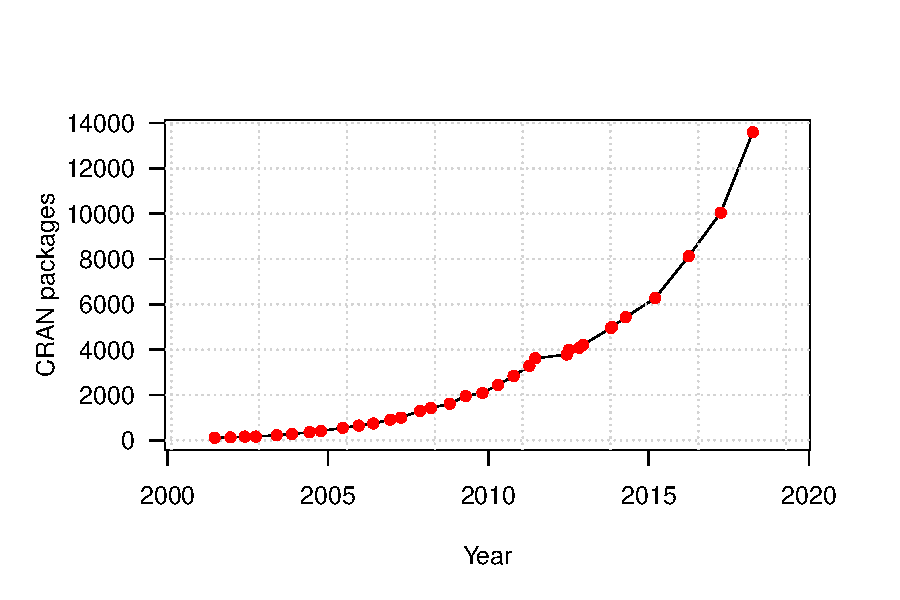
\includegraphics[width=0.7\textwidth]{figura13.pdf}
\caption[Number of R packages on CRAN since 2002]{Number of R packages on CRAN has been growing at an exponential rate since 2002.}
\label{figura13}
\end{figure}

With the huge number of packages at the disposal of \texttt{R} users, many advanced functions have already been programmed and are available for they use or reuse when programming new functionalities. Apart from the main repository (CRAN) there are other important repositories with thousands of packages more such as \textit{R-Forge}, \textit{Bioconductor} or even \textit{Github}. All this functionallity and the fact that R is open source motivated the election of \texttt{R} as the language for developing all the techniques and tools presented in this thesis.

\subsection{\texttt{R} packages for the analysis of three-way data}
Most three-way data procedures are implemented in MATLAB\textsuperscript{\tiny\textregistered} \textcite{MATLAB:2010} (or previous versions of the software). Concretely, the $N$-way toolbox by \textcite{andersson2000n} provides a comprehensive set of functions for dealing with three- and multi-way arrays in MATLAB\textsuperscript{\tiny\textregistered}. \texttt{R}, on the other hand, only has two packages dedicated to the analysis of three- or multi-way data. The packages \texttt{PTAk} \parencite{leibovici2010spatio} and \texttt{ThreeWay} \parencite{giordani2014three}, offer a suit of functions for handling three-way arrays in \texttt{R}. These functions include Tucker3 and PARAFAC models and also some processing methods for three-way data such as centering, scaling, unfolding and normalizing arrays. However, $N$-PLS is notably missing from these packages, so no prediction method for three-way arrays was implemented in \texttt{R} before the release of our \texttt{sNPLS} package presented in this section. In this way, with the development of the package, we have not only implemented a newly developed method such as sparse $N$-PLS, but also enabled the use of standard $N$-PLS regression models to \texttt{R} users.


\section{Implementation of the sNPLS algorithm in \texttt{R}}
In this section the key functions of the code for the \textit{sNPLS} package will be exposed and commented. These include the main sNPLS function, the R-matrix function and the cross-validation functions. The full code for the package will be included in the appendix.

\subsection{Main algorithm}
This is the code of the main function of the package. It performs $N$-PLS regression as explained in \autoref{NPLSregression} and includes an L1-penalization step at the determination of $\textbf{\text{w}}^{J}$ and $\textbf{\text{w}}^{K}$ as explained in \autoref{NPLSpenalization}.
\vspace{15pt}
\begin{scriptsize}
\begin{lstlisting}[language=R, deletekeywords={scale, !=, <-, !, Q, qf, names, max, var}, otherkeywords={}, morekeywords={unfold3w}, caption=sNPLS main function]
sNPLS <- function(XN, Y, ncomp = 2, conver = 1e-16, max.iteration = 10000,
                  keepJ = rep(ncol(XN), ncomp), 
                  keepK = rep(rev(dim(XN))[1], ncomp),
                  scale.X=TRUE, center.X=TRUE, scale.Y=TRUE, center.Y=TRUE, 
                  silent = F) {
  
  mynorm <- function(x) sqrt(sum(diag(crossprod(x))))
  if (length(dim(Y)) == 3) Y <- unfold3w(Y)
  if (length(dim(XN)) != 3)
    stop("'XN' is not a three-way array")
  if (!is.null(rownames(XN)))
    y.names <- x.names <- rownames(XN) else {
    y.names <- x.names <- 1:dim(XN)[1]
    }
    if (!is.null(colnames(XN)))
      var.names <- colnames(XN) else {
      var.names <- paste("X.", 1:dim(XN)[2], sep = "")
      }
      if (!is.null(dimnames(XN)[[3]]))
        x3d.names <- dimnames(XN)[[3]] else {
        x3d.names <- paste("Z.", 1:dim(XN)[3], sep = "")
        }
        if (!is.null(colnames(Y)))
          yvar.names <- colnames(Y) else {
          yvar.names <- paste("Y.", 1:dim(Y)[2], sep = "")
          }
          if(!center.X) center.X <- rep(0, ncol(XN)*dim(XN)[3])
          if(!center.Y) center.Y <- rep(0, ncol(Y))
          if(!scale.X) scale.X <- rep(1, ncol(XN)*dim(XN)[3])
          if(!scale.Y) scale.Y <- rep(1, ncol(Y))
          
          # Matrices initialization
          Tm <- U <- Q <- WsupraJ <- WsupraK <- X <- P <- NULL
          Yorig <- Y
          Y <- scale(Y, center = center.Y, scale = scale.Y)
          y_center <- attr(Y, "scaled:center")
          y_scale <- attr(Y, "scaled:scale")
          B <- matrix(0, ncol = ncomp, nrow = ncomp)
          Gu <- vector("list", ncomp)
          S <- svd(Y)$d
          u <- Y[, S == max(S)]  #Column with the highest variance
          # Unfolding of XN en 2-D
          X <- unfold3w(XN)
          #Check for zero variance columns and fix them with some noise
          if(any(apply(X, 2, sd)==0)){
            X[,apply(X, 2, sd)==0] <- apply(X[,apply(X, 2, sd)==0, drop=F], 
                                            2, function(x) jitter(x))
          }
          # Center and scale
          Xd <- scale(X, center = center.X, scale = scale.X)
          x_center <- attr(Xd, "scaled:center")
          x_scale <- attr(Xd, "scaled:scale")
          
          # Main loop for each component
          for (f in 1:ncomp) {
            nj <- ncol(XN) - keepJ[f]
            nk <- dim(XN)[3] - keepK[f]
            it = 1
            while (it < max.iteration) {
              Zrow <- crossprod(u, Xd)
              Z <- matrix(Zrow, nrow = dim(XN)[2], ncol = dim(XN)[3])
              svd.z <- svd(Z)
              wsupraj <- svd.z$u[, 1]
              # L1 penalization for wsupraj
              if (nj != 0) {
                wsupraj <- ifelse(abs(wsupraj) > 
                                  abs(wsupraj[order(abs(wsupraj))][nj]),
                                  (abs(wsupraj) - 
                                  abs(wsupraj[order(abs(wsupraj))][nj])) *
                                  sign(wsupraj), 0)
              }
              ##########
              wsuprak <- svd.z$v[, 1]
              # L1 penalization for wsuprak
              if (nk != 0) {
                wsuprak <- ifelse(abs(wsuprak) > 
                                  abs(wsuprak[order(abs(wsuprak))][nk]),
                                  (abs(wsuprak) - 
                                  abs(wsuprak[order(abs(wsuprak))][nk])) *
                                  sign(wsuprak), 0)
              }
              ##########
              tf <- Xd %*% kronecker(wsuprak, wsupraj)
              qf <- crossprod(Y, tf)/mynorm(crossprod(Y, tf))
              uf <- Y %*% qf
              if (sum((uf - u)^2) < conver) {
                if (!silent) {
                  cat(paste("Component number ", f, "\n"))
                  cat(paste("Number of iterations: ", it, "\n"))
                }
                it <- max.iteration
                Tm <- cbind(Tm, tf)
                WsupraJ <- cbind(WsupraJ, wsupraj)
                WsupraK <- cbind(WsupraK, wsuprak)
                bf <- MASS::ginv(crossprod(Tm)) %*% t(Tm) %*% uf
                B[1:length(bf), f] <- bf
                Q <- cbind(Q, qf)
                U <- cbind(U, uf)
                TM <- MASS::ginv(crossprod(Tm)) %*% t(Tm)
                WkM <- MASS::ginv(crossprod(WsupraK)) %*% t(WsupraK)
                WjM <- MASS::ginv(crossprod(WsupraJ)) %*% t(WsupraJ)
                Gu[[f]] <- TM %*% X %*% kronecker(t(WkM), t(WjM))
                P[[f]] = t(as.matrix(Gu[[f]]) %*% 
                         t(kronecker(WsupraK, WsupraJ)))
                Y <- Y - Tm %*% bf %*% t(qf)
                S <- svd(Y)$d
                u <- Y[, S == max(S)]
              } else {
                u <- uf
                it <- it + 1
              }
            }
          }
          Yadjsc <- Tm %*% B %*% t(Q)
          Yadj <- Yadjsc * y_scale + y_center
          SqrdE <- sum((Yorig - Yadj)^2)
          rownames(WsupraJ) <- var.names
          rownames(WsupraK) <- x3d.names
          rownames(Q) <- yvar.names
          rownames(Tm) <- rownames(U) <- x.names
          colnames(Tm) <- colnames(WsupraJ) <- colnames(WsupraK) <- 
                          colnames(B) <- colnames(U) <- colnames(Q) <- 
                          names(Gu) <- names(P) <- paste("Comp.", 1:ncomp)
          output <- list(T = Tm, Wj = WsupraJ, Wk = WsupraK, B = B, U = U, 
                         Q = Q, P = P, Gu = Gu, ncomp = ncomp, Yadj = Yadj, 
                         SqrdE = SqrdE, 
                         Standarization = list(ScaleX = x_scale, 
                                               CenterX = x_center,
                                               ScaleY = y_scale, 
                                               CenterY = y_center))
          class(output)<-"sNPLS"
          return(output)
}
\end{lstlisting}
\end{scriptsize}

Lines 1-5 define the parameters of the function. Parameters with default values have that value assigned after an equal sign. Line 7 defines an internal function for normalization. Lines 8-30 check for inconsistencies in the data structure, unfold \textbf{\underline{Y}} (when necessary) and assign variable names. After this, all necessary matrices are initiallized in lines 33-52, \textbf{\underline{X}} is unfolded into \textbf{X} and optional centering and scaling is applied on \textbf{Y} and \textbf{X}. The following lines (55-113) correspond to the $N$-PLS algorithm described in \autoref{NPLSpenalization}. Last lines (114-133) include the estimation of \textbf{Y}, the computing of the squared prediction error, and the generation of the output object of the function, defined as an S3 object of class \textit{sNPLS}. This object includes the different output matrices of the model as well as all the information regarding the model fit such as centering on \textbf{X} and/or \textbf{Y} and used values for the hyperparameters. 


\subsection{R matrix computation}
\label{rmatrixf}
This function is used for computing the coefficients used for prediction of \textbf{Y} in the \texttt{predic.sNPLS} function.
\vspace{15pt}
\begin{scriptsize}
\begin{lstlisting}[language=R, deletekeywords={scale, !=, <-, !, Q, qf, names, max, var}, otherkeywords={}, morekeywords={unfold3w}, caption=R matrix function]
Rmatrix<-function(x) {
  WsupraK <- x$Wk
  WsupraJ <- x$Wj
  R <- matrix(nrow = dim(x$Wj)[1] * dim(x$Wk)[1], ncol = x$ncomp)
  ncomp <- x$ncomp
  kroneckers<-sapply(1:x$ncomp, function(x) {
                     kronecker(WsupraK[, x], WsupraJ[, x]))
                     }
  tkroneckers<-apply(kroneckers, 2, function(x) t(x))
  R[,1] <- kroneckers[,1]
  if(ncomp>1){
    for(i in 2:ncomp){
      pi <- pi0 <- Matrix::Matrix(diag(dim(R)[1]), sparse=TRUE)
      for (j in 1:(i - 1)) {
        pi <- Matrix::Matrix(pi %*% pi0 - kroneckers[,j] %*% 
        t(tkroneckers[,j]), sparse=TRUE)
      }
      w <- kroneckers[, i]
      pi <- pi %*% w
      R[, i] <- Matrix::as.matrix(pi)
    }
  }
  return(R)
}
\end{lstlisting}
\end{scriptsize}

Of note, most of the computations performed inside the \texttt{Rmatrix} function make use of sparse matrices (lines 12-19), taking advantage of the sparsity created by the \texttt{sNPLS} function when adjusting the model to greatly reduce computing times. The \texttt{Rmatrix} function is an internal function (not exported to the end user) called by the \texttt{sNPLS} and \texttt{predict.sNPLS} functions to get the regression coefficients in order to be able to perform predictions from new \textbf{\underline{X}} as explained in \textcite{leardi2005multi}:

The \textbf{R} matrix is defined as:

\begin{equation}
    \textbf{\text{R}}=[\textbf{\text{w}}_1(\textbf{\text{I}}-\textbf{\text{w}}_1\textbf{\text{w}}^T_1)\textbf{\text{w}}_2 \dots (\prod_{f=1}^{F-1}(\textbf{\text{I}}-\textbf{\text{w}}_f\textbf{\text{w}}^T_f)\textbf{\text{w}}_F)]
\end{equation}

From this, it derives that

\begin{equation}
    \textbf{\text{T}}=\textbf{\text{XR}}
\end{equation}

So, from the equation

\begin{equation}
    \hat{\textbf{\text{y}}}=\textbf{\text{Tb}}
\end{equation}

We obtain

\begin{equation}
    \textbf{\text{b}}_{NPLS}=\textbf{\text{Rb}}
\end{equation}

\subsection{Cross validation (\texttt{cv\_snpls})}
The \texttt{cv\_snpls} function is used to estimate the best combination of parameters for adjusting sNPLS models using $K$-fold cross-validation. Since the hyperparameter space can be huge when considering a grid search for three different hyperparameters, it has been parallelized using the \textit{parallel} package to greatly speed up computation times. For simple problems or small data sets it can also be run in single thread mode.
\vspace{15pt}
\begin{scriptsize}
\begin{lstlisting}[language=R, deletekeywords={scale, !=, <-, !, Q, qf, names, max, var, drop, se, search.grid, mean, grid, search}, otherkeywords={}, morekeywords={unfold3w}, caption=Cross validation function]
cv_snpls <- function(X_npls, Y_npls, ncomp = 1:3, keepJ = 1:ncol(X_npls),
                     keepK = 1:dim(X_npls)[3], nfold = 10, parallel = TRUE, 
                     free_cores = 2, ...) {
    #Creation of cluster and exportation of data to the nodes
    if (parallel & (parallel::detectCores()>1)) {
        cl <- parallel::makeCluster(max(2, 
                                    parallel::detectCores() - free_cores))
        parallel::clusterExport(cl, list(deparse(substitute(X_npls)),
                                         deparse(substitute(Y_npls))))
        parallel::clusterCall(cl, function() require(sNPLS))
    }
  if(length(dim(Y_npls)) == 3) Y_npls <- unfold3w(Y_npls)
  top <- ceiling(dim(X_npls)[1]/nfold)
    foldid <- sample(rep(1:nfold, top), dim(X_npls)[1], replace = F)
    #Expansion of hyperparameters grid
    search.grid <- expand.grid(list(ncomp = ncomp, 
                                    keepJ = keepJ, 
                                    keepK = keepK))
    SqrdE <- numeric()
    #Main function
    applied_fun <- function(y) {
        sapply(1:nfold, function(x) {
            tryCatch(cv_fit(xtrain = X_npls[x != foldid, , ],
                            ytrain = Y_npls[x != foldid, , drop = FALSE],
                            xval = X_npls[x == foldid, , ],
                            yval = Y_npls[x == foldid, , drop = FALSE],
                            ncomp = y["ncomp"],
                            keepJ = rep(y["keepJ"], y["ncomp"]),
                            keepK = rep(y["keepK"], y["ncomp"]), ...),
                     error=function(x) NA)
          })
    }
    #Parallelization of main function
    if (parallel) {
        cv_res <- parallel::parApply(cl, search.grid, 1, applied_fun)
        parallel::stopCluster(cl)
    } else cv_res <- pbapply::pbapply(search.grid, 1, applied_fun)
    cv_mean <- apply(cv_res, 2, function(x) mean(x, na.rm = TRUE))
    cv_se <- apply(cv_res, 2, function(x) sd(x, na.rm=TRUE)/sqrt(nfold))
    best_model <- search.grid[which.min(cv_mean), ]
    output <- list(best_parameters = best_model, cv_mean = cv_mean,
                   cv_se = cv_se, cv_grid = search.grid)
    class(output)<-"cvsNPLS"
    return(output)
}
\end{lstlisting}
\end{scriptsize}

Of note, regarding the \texttt{cv\_snpls} function, is the code related to the parallelization of the procedure using the \texttt{parallel} package (lines 5-11 for the definition of the cluster and lines 34-37 for the execution of the parallelized procedure). The function makes use of the \texttt{parApply} function, which splits the search grid in $n$ nodes and runs the cross-validation procedure on each split independently, combining all results at the end of the computations. Lines 21-32 of the function correspond to the cross-validation procedure defined in \autoref{hyperparameters}.

\subsection{Repeated Cross validation (\texttt{repeat\_cv})}
\label{repeatcv}
The \texttt{repeat\_cv} calls the \texttt{cv\_snpls} function repeated times, but it changes the way of parallelizing the computations. 

In this function, each \texttt{cv\_snpls} call is run in single thread mode, but assigned to a different node. So, instead on subsets of the search grid, the parallelization is performed on repetitions of the procedure on the whole grid. This handling of the parallelization allows for a more efficient distribution of the jobs across the different nodes of the defined cluster, assuming the number of repetitions is greater than the number of folds $K$ of the $K$-fold cross-validation procedure.

\vspace{12pt}
\begin{lstlisting}[language=R, deletekeywords={scale, !=, <-, !, Q, qf, names, max, var, drop, se, search.grid, mean, grid, search, rep, repeat}, otherkeywords={}, morekeywords={unfold3w, pbreplicate, parSapply}, caption=Repeated cross validation function]
repeat_cv<-function(X_npls, Y_npls, ncomp = 1:3, keepJ = 1:ncol(X_npls), 
                    keepK = 1:dim(X_npls)[3], nfold = 10, 
                    parallel = TRUE, free_cores = 2, times=30, ...){
  #Definition of the cluster and exportation of data to the nodes
  if(parallel & (parallel::detectCores()>1)){
    cl <- parallel::makeCluster(max(2, 
                                parallel::detectCores() - free_cores))
    parallel::clusterExport(cl, list(deparse(substitute(X_npls)), 
                                     deparse(substitute(Y_npls))))
    parallel::clusterCall(cl, function() require(sNPLS))
    #Parallelization of the repetitions of K-fold cross-validation
    rep_cv<-parallel::parSapply(cl, 1:times, function(x){
                                cv_snpls(X_npls, Y_npls, ncomp=ncomp, 
                                keepJ = keepJ, keepK = keepK, 
                                parallel = FALSE, nfold = nfold, ...))
                                }
    parallel::stopCluster(cl)
  } else {
    #Single threaded version (Not use, slow)
    rep_cv<-pbapply::pbreplicate(times, cv_snpls(X_npls, Y_npls, 
                                 ncomp=ncomp, keepJ = keepJ, 
                                 keepK = keepK, parallel = FALSE, 
                                 nfold = nfold, ...))
  }
  resdata<-data.frame(ncomp=sapply(rep_cv[1,], function(x) x[[1]]), 
                      keepJ=sapply(rep_cv[1,], function(x) x[[2]]),
                      keepK=sapply(rep_cv[1,], function(x) x[[3]]))
  class(resdata)<-c("repeatcv", "data.frame")
  return(resdata)
}
\end{lstlisting}

\section{The sNPLS package}
In the following section, the use of the different functions of the \texttt{sNPLS} package will be presented, as well as examples of their application to the different parts of the analysis in two data sets. A special emphasis will be given to the main \texttt{sNPLS} function, as well as to both cross-validation functions for the selection of the hyperparameters and to the different plot functions for the interpretation of results. This section is based on our published paper for the \textit{sNPLS} package \parencite{hervas2018sparse}.

\subsection{Functions}
\subsubsection{\texttt{sNPLS} function}
Function \texttt{sNPLS} is used to fit $N$-PLS and sNPLS models to three-way data, depending on the input settings of the algorithm. The following \textit{R} code shows an example of a model fit to a simulated three-way dataset with fifty observations ($I$), 50 variables ($J$) and three elements in the third mode ($K$).
\vspace{15pt}
\begin{lstlisting}[basicstyle=\small, language=Python, morekeywords={array, matrix, sNPLS, rep, rpois, rnorm}]
R> library("sNPLS")
R> X_npls <- array(rpois(7500, 10), dim=c(50, 50, 3))
R> Y_npls <- matrix(2+0.4*X_npls[,5,1]+0.7*X_npls[,10,1]- 
+    0.9*X_npls[,15,1] + 0.6*X_npls[,20,1] - 0.5*X_npls[,25,1]+
+    rnorm(50), ncol=1)
R> fit <- sNPLS(X_npls, Y_npls, ncomp=3, keepJ = rep(2,3), 
+    keepK = rep(1,3))
\end{lstlisting}

Note that the function \texttt{sNPLS} needs a $N$-way array for \textbf{\underline{X}} and an $N$-way array, a two-dimensional matrix or a numeric vector for \textbf{Y} as inputs. If data is in another format the function will stop and throw an error. In the following paragraph, a generic call with a short description of each of the arguments of the function is presented.
\vspace{15pt}
\begin{lstlisting}[basicstyle=\small, language=R, deletekeywords={max, scale}, morekeywords={array, matrix, rep, rpois, rnorm, function}, otherkeywords={}]
sNPLS(XN, Y, ncomp = 2, conver = 1e-16, 
+    max.iteration = 10000, keepJ = rep(ncol(XN), ncomp), 
+    keepK = rep(rev(dim(XN))[1], ncomp), scale.X=TRUE, 
+    center.X=TRUE, scale.Y=TRUE, center.Y=TRUE, silent = F)
\end{lstlisting}
\vspace{10pt}
\begin{itemize}[leftmargin=2.5cm]
\item[XN] $N$-dimensional array containing the predictors
\item[Y] Array containing the response(s)
\item[ncomp] Number of components to use in the projection
\item[conver] Convergence criterion
\item[max.iteration] Maximum allowed number of iterations to achieve convergence
\item[keepJ] Number of variables to keep at each component. If all variables are kept, NPLS regression is performed, if any variable is removed then sNPLS is performed.
\item[keepK] Number of elements of the third mode to keep at each component.
\item[scale.X] Perform scaling on \textbf{\text{X}}?
\item[center.X] Perform centering on \textbf{\text{X}}?
\item[scale.Y] Perform scaling on \textbf{\text{Y}}?
\item[center.Y] Perform centering on \textbf{\text{Y}}?
\item[silent] Allows to choose if information regarding number of iterations should be displayed
\end{itemize}
\vspace{7pt}
The function \texttt{sNPLS} produces an \texttt{S3 sNPLS} object with defined \texttt{coef}, \texttt{predict} and \texttt{plot} methods that will be discussed later. The object consists of a list containing the following components: [1-6] The \textbf{T}, $\textbf{\text{W}}^{J}$, $\textbf{\text{W}}^{K}$, \textbf{B} (regression coefficients between \textbf{\underline{X}} and \textbf{\underline{Y}}), \textbf{Y} and \textbf{Q} matrices, [7-8] \textbf{P} and \textbf{G}u (the unfolded \textbf{G} core array of the Tucker decomposition), [9] The number of components, [10] Fitted values, [11] Squared error, [12] Scale and centering information performed on \textbf{\underline{X}} and \textbf{Y}.

\subsubsection{\texttt{cv\_sNPLS} and \texttt{repeat\_cv} functions}
Selecting parameter values for the \texttt{sNPLS} function requires choosing values for the number of components, the number of variables to select and the number of elements of the third mode to select. An appropriate way of selecting these parameters is performing a grid search with cross-validation. The function \texttt{cv\_snpls} performs cross-validation on a grid of different \texttt{ncomp}, \texttt{keepJ} and \texttt{keepK} values estimating $RMSE$ (Root Mean Square Error) for each combination of values and selecting the best set producing the lowest $RMSE$.

\vspace{15pt}
\begin{lstlisting}[basicstyle=\small, language=Python, deletekeywords={max, scale}, morekeywords={array, matrix, rep, rpois, rnorm, function, cv_snpls}, otherkeywords={}]
R> X_npls<-array(rpois(7500, 10), dim=c(50, 50, 3))
R> Y_npls<-matrix(2+0.4*X_npls[,5,1]+0.7*X_npls[,10,1]-
+    0.9*X_npls[,15,1]+0.6*X_npls[,20,1]- 0.5*X_npls[,25,1]+
+    rnorm(50), ncol=1)
R> cv1<- cv_snpls(X_npls, Y_npls, ncomp=1:2, keepJ = 1:10, 
+    keepK = 1:3, parallel = FALSE)
\end{lstlisting}

The generic call for \texttt{cv\_snpls} is the following:
\vspace{15pt}
\begin{lstlisting}[basicstyle=\small, language=R, deletekeywords={max, scale}, morekeywords={array, matrix, rep, rpois, rnorm, function, cv_snpls}, otherkeywords={}]
cv_snpls(X_npls, Y_npls, ncomp = 1:3, keepJ = 1:ncol(X_npls),
+   keepK = 1:dim(X_npls)[3], nfold = 10, parallel = FALSE)
\end{lstlisting}

It contains the same parameters as \texttt{sNPLS} but now admits vectors of values for each parameter in \texttt{ncomp}, \texttt{keepJ} and \texttt{keepK}. Since grid search can be computationally intensive, it makes use of the \texttt{parallel} package. Being able to perform computations in parallel greatly reduces running times, being able to finish between 1.5 and 6 times faster in an eight-core computer, depending on the data set. Parallel mode is activated by setting \texttt{parallel} argument to \texttt{TRUE} and selecting a suitable number of free cores. As explained in \autoref{repeatcv}, in the case of \texttt{cv\_snpls}, the parallelization applies to the grid search, not to the different folds of the cross-validation.

To further reduce computation times and improve memory use, sparse matrices from the \texttt{R} package \texttt{Matrix} \parencite{matrixsparse} are used whenever possible in the matrix multiplication steps of the function. Sparse matrices achieve these goals by using an alternative representation to that of dense matrices: instead of being stored as two-dimensional arrays, only their non-zero values are stored, along with an index linking these values with their location in the matrix. The function \texttt{cv\_snpls} returns a \texttt{cvsnpls} object which is a list with a component containing the best combination parameters and other components containing information about the grid and its corresponding \texttt{RMSE}. \texttt{cv\_snpls} objects  can be plotted for better interpretation of the results. The resulting plot is a grid of scatterplots with the different combinations of \texttt{keepJ}, \texttt{keepK} and \texttt{ncomp} and their resulting cross-validation errors (\autoref{figura04}).

\vspace{10pt}
\begin{figure}[!ht]
	\centering
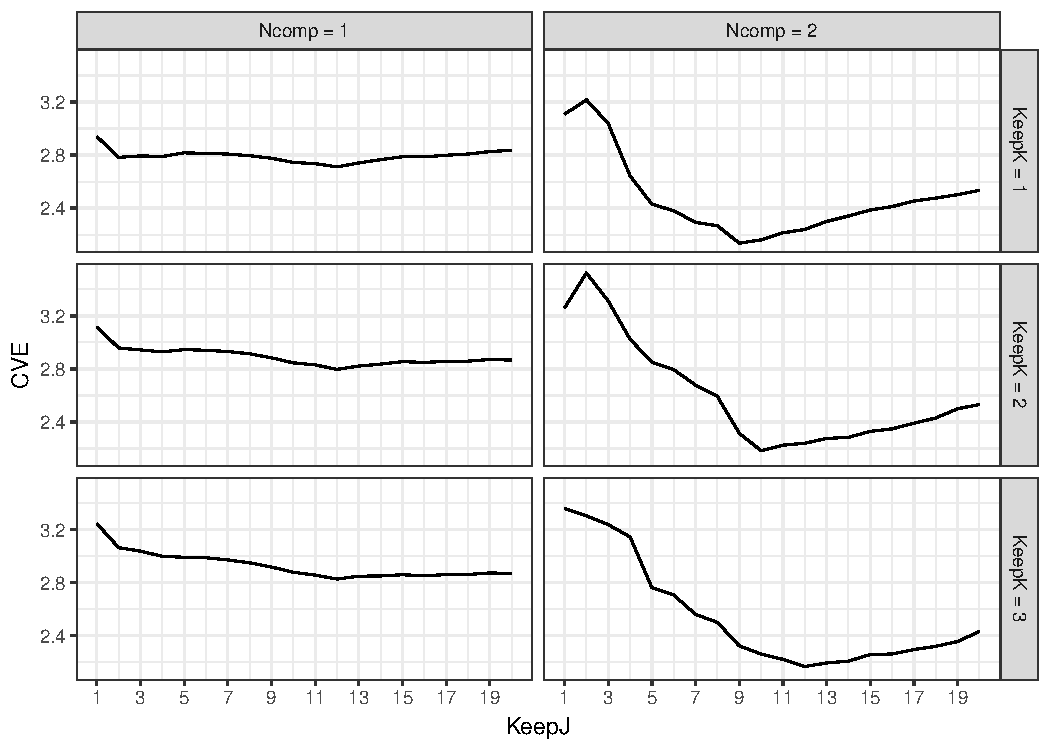
\includegraphics[width=0.85\textwidth]{figura04.pdf}
\caption[Results of cross-validation]{Results of cross-validation. Lines depicting the cross-validated error (CVE) for each combination of the parameters are presented in a grid layout combining \texttt{KeepJ} values (number of variables selected), \texttt{KeepK} values (number of elements of the third mode) and \texttt{Ncomp} values (number of components).}
\label{figura04}
\end{figure}
\vspace{10pt}

A known issue of cross-validation is the variance in its results \parencite{krstajic2014cross}, which entails that different runs of the cross-validation procedure can yield different results regarding the estimated best set of parameters and, more importantly, that the cross-validation procedure can overfit in the estimation of the error. This overfitting would entail that repeating the same cross-validation procedure on another sample of the population would yield totally different results. A reasonable solution is performing repeated cross-validation and selecting the most frequently selected set of parameters along a round of different runs. The function \texttt{repeat\_cv} performs repeated cross-validation by calling the function \texttt{cv\_snpls} repeated times and storing each result in a \texttt{data.frame} object. The syntax is the same as in \texttt{cv\_snpls} with an extra argument \texttt{times} for specifying the number of repetitions to perform. In the case of \texttt{repeat\_cv} the parallelization applies to the replicates instead of applying to the grid search. The following code explains how to perform repeated cross-validation with \texttt{repeat\_cv}.

\vspace{15pt}
\begin{lstlisting}[basicstyle=\small, language=Python, deletekeywords={max, scale}, morekeywords={array, matrix, rep, rpois, rnorm, function, repeat_cv}, otherkeywords={}]
R> repcv <- repeat_cv(X_npls, Y_npls, ncomp=1:2, keepJ = 1:10, 
+    keepK = 1:3, parallel = FALSE, times=10)
\end{lstlisting}

The result of the \texttt{repeat\_cv} call is a \texttt{data.frame} storing the results (best combination of \texttt{ncomp}, \texttt{keepJ} and \texttt{keepK} of each cross-validation repetition (\autoref{output1}). 

\vspace{15pt}
\begin{lstlisting}[basicstyle=\small, language=Python]
R> repcv
\end{lstlisting}

\vspace{5pt}
\begin{lstlisting}[basicstyle=\small, backgroundcolor=\color{output}, numbers=none, label={output1}, language=Python, caption=Results of \texttt{repeat\_cv} function.]
   ncomp keepJ keepK
1      2     9     1
2      2     9     1
3      2    10     1
4      2     9     1
5      2    11     2
6      2    12     1
7      2     7     1
8      2    10     1
9      2     8     1
10     2    12     2
\end{lstlisting}

This output can be presented as a cross-tabulation table with the absolute frequencies of each combination of the different parameters (\autoref{output2}. In our example, the table shows that the combination \texttt{ncomp}=2, \texttt{keepJ}=9 and \texttt{keepK}=1 is the most recurrent (3 out of 10 repetitions), followed by the combination \texttt{ncomp}=2, \texttt{keepJ}=10 and \texttt{keepK}=1 with two repetitions and five other different combinations with just one occurrence each. It can also be noticed that none of the best combinations included only one component.

\vspace{15pt}
\begin{lstlisting}[basicstyle=\small, language=Python, deletekeywords={max, scale}, morekeywords={ftable, table}, otherkeywords={}]
R> ftable(table(repcv))
\end{lstlisting}

\begin{lstlisting}[basicstyle=\small, backgroundcolor=\color{output}, numbers=none, label={output2}, language=Python, caption=Cross-tabulation table of the results of \texttt{repeat\_cv}.]
            keepK 1 2
ncomp keepJ          
2     7           1 0
      8           1 0
      9           3 0
      10          2 0
      11          0 1
      12          1 1
\end{lstlisting}

Results of the \texttt{repeat\_cv} function can also be plotted to obtain a kernel density plot, which can be one-, two- or three-dimensional depending of the number of constant parameters obtained in the repeated cross-validation procedure. This density plot depicts the most frequently selected parameters (\autoref{figura05}). 
\vspace{10pt}
\begin{figure}[hbtp]
	\centering
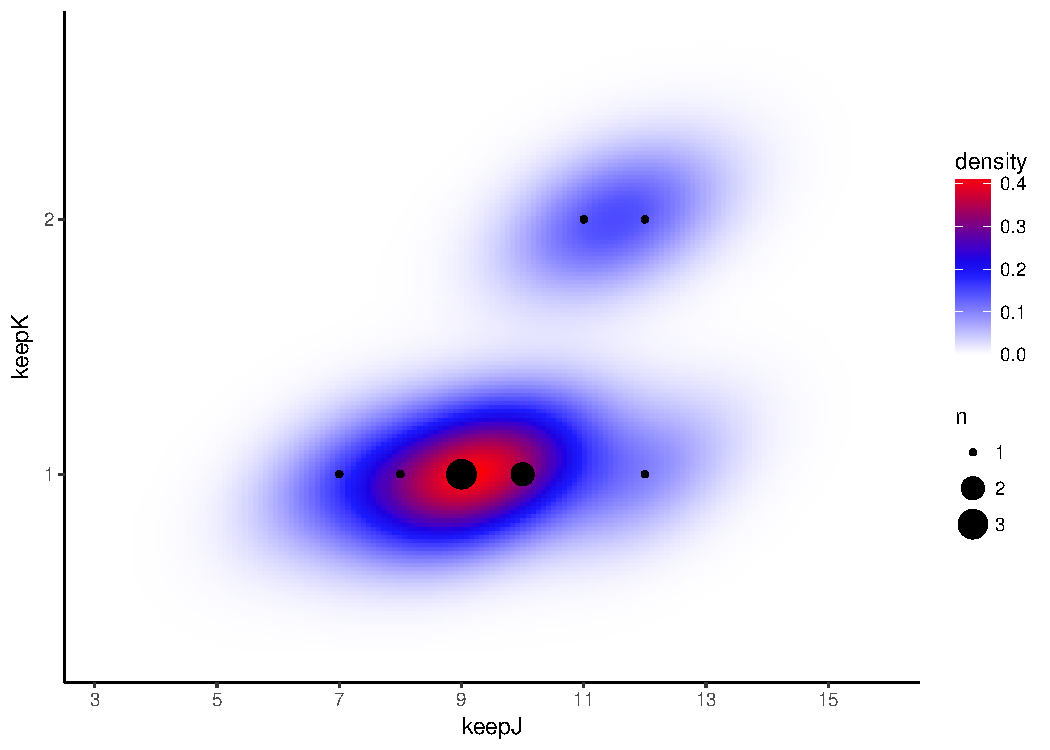
\includegraphics[width=0.7\textwidth]{figura05.pdf}
\caption[Kernel density plot with the results of repeated cross-validation]{Kernel density plot with the result of the repeated cross-validation. Highest density lies around \texttt{keepJ}=9 and \texttt{keepK}=1. Points scaled in size by frequency of appearance are additionally included on top of the density plot. The number of components is not represented since it was constant at 2 in all repetitions of the cross-validation.}
\label{figura05}
\end{figure}

In this example, according to the plot, the most likely combination after all repetitions of the cross-validation was between 9 and 10 in the case of \texttt{keepJ} and \texttt{keepK}=1. Since the optimal number of components did not vary along all the repetitions, this parameter is not represented in the plot. Instead, the message \texttt{'ncomp is(are) constant with a value of 2'} is returned by the function. The density plot leads to a similar interpretation of the results as the cross-tabulation table, but the smoothing can result in more sensible estimates in the case of multiple and/or wide spread modes. It also provides a visual measure of the uncertainty in the selection of the best combination of parameters.

\subsubsection{Full example functionality}
To exhibit all package functionality, next we provide a complete analysis of the \texttt{bread} dataset \parencite{bro1998multi} included in the \textit{sNPLS} package. This data set consists on data of five different breads that were baked in duplicate giving a total of ten samples. Eight different judges assessed the breads with respect to eleven different sensorial attributes. The data can be regarded as a three-way array (10 x 11 x 8). The data are quite noisy as opposed to, e.g., spectral data. The salt content of each bread was also measured and it is considered as the response variable \textbf{y}.
\vspace{15pt}
\begin{lstlisting}[basicstyle=\small, language=Python, morekeywords={data, repeat_cv}]
R> data(bread)
R> Xbread <- bread$Xbread
R> Ybread <- bread$Ybread
R> cv_bread <- repeat_cv(Xbread, Ybread, ncomp=1:3, keepJ = 1:11,   
+    keepK = 1:8, parallel = FALSE, times=50, nfold=3)
\end{lstlisting}

After importation of the data set and preparation of the \textbf{\underline{X}} array and \textbf{y} vector (first three lines of the code above), repeated cross-validation is performed on the data to select the optimal combination of hyperparameters. 50 repetitions of 3-fold cross-validation should be enough to get stable estimates, but using such a large number of repetitions would increase computing times dramatically. Therefore, using the option \texttt{parallel=TRUE} when performing repeated cross-validation is recommended. Results of this procedure yield a cross-tabulation table with the appearance frequencies for each combination of parameters \autoref{output3}.

\vspace{15pt}
\begin{lstlisting}[basicstyle=\small, language=Python, morekeywords={ftable, table}]
R> ftable(table(cv_bread)) 
\end{lstlisting}

\begin{lstlisting}[basicstyle=\small, backgroundcolor=\color{output}, numbers=none, label={output3}, language=Python, caption=\texttt{repeat\_cv} results for the \texttt{bread} data set.]
            keepK 1 2 3 4 5 6 7 8
ncomp keepJ                      
1     1           1 2 2 4 3 3 1 1
      2           0 0 1 1 2 1 0 2
2     1           0 0 0 0 0 0 0 1
      2           0 0 0 0 0 0 0 2
      3           0 0 0 0 0 1 0 4
      4           0 0 0 0 0 0 1 1
      5           1 0 0 0 0 0 0 1
      6           0 0 0 0 0 0 1 0
      7           0 0 0 0 0 0 1 0
      8           0 0 0 0 0 0 0 2
      9           0 0 0 0 0 0 0 1
3     1           0 0 1 0 0 2 0 1
      2           0 0 0 0 0 0 1 1
      3           0 0 0 0 0 0 0 1
      5           0 0 0 0 0 0 0 1
\end{lstlisting}    
      
This table shows that there are two possible combinations of parameters that are almost equally selected by cross-validation. One is \texttt{ncomp}=1, \texttt{keepJ}=1 and \texttt{keepK}=4 and the other is \texttt{ncomp}=2, \texttt{keepJ}=3 and \texttt{keepK}=8, both with 4 appearances out of 50 repetitions. Also most of the other combinations are close to one of these two mentioned 'hotspots'. A plot of the \texttt{cv\_bread} object (\autoref{figura06}) reveals a similar information with a representation of a sliced three-dimensional kernel density estimate.


\begin{figure}[!ht]
	\centering
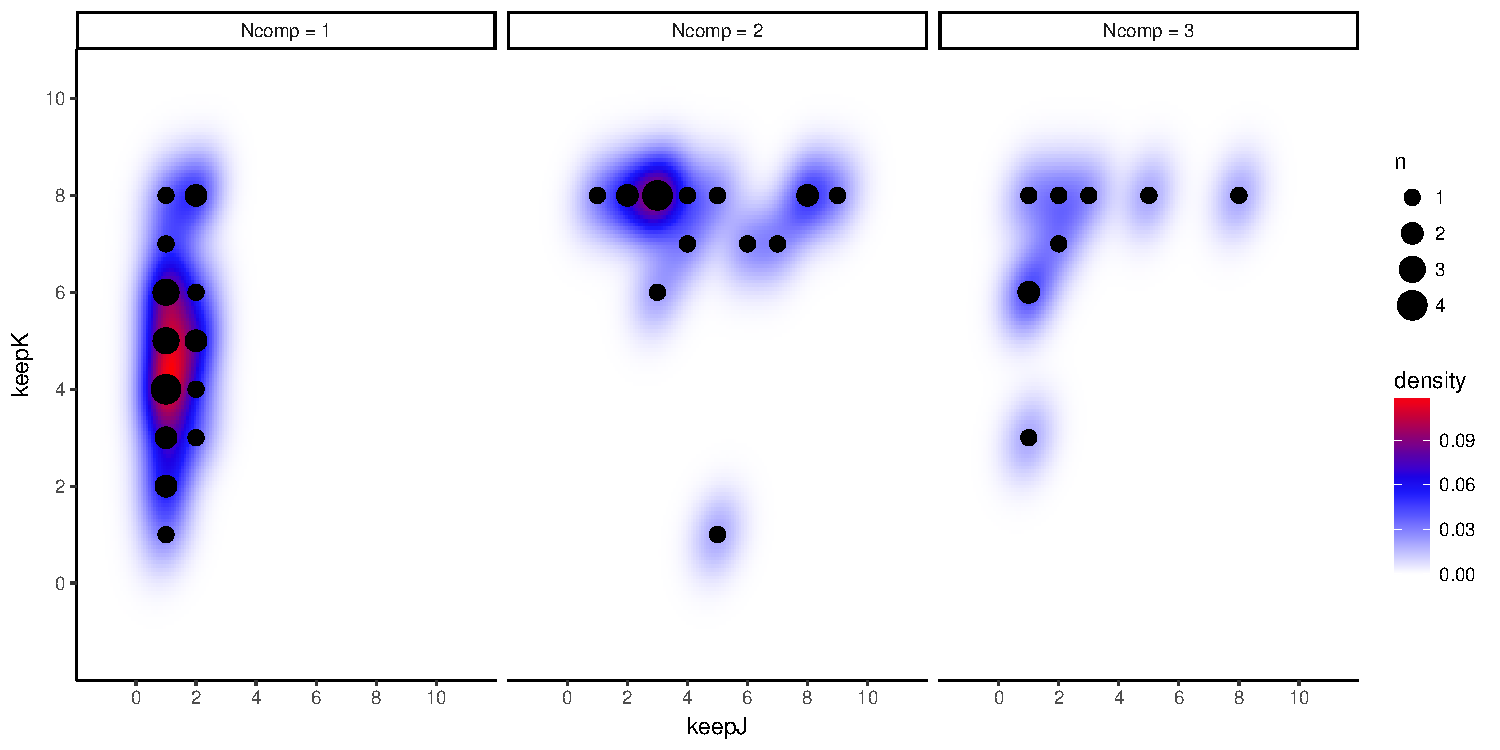
\includegraphics[width=0.98\textwidth]{figura06.pdf}
\caption[Results of the repeated cross-validation function performed on the \texttt{bread} dataset]{Results of the repeated cross-validation function performed on the \texttt{bread} dataset. The plot consists on the faceted representation of a three-dimensional density plot sliced in different planes (one per number of components). The kernel density estimation is created with the observed frequencies of the combinations of the different parameters. Additionally, points scaled in size by frequency of appearance are added to the density plots.}
\label{figura06}
\end{figure}

Next step would be fitting the \texttt{sNPLS} model using the \texttt{sNPLS} function with the selected set of parameters. As discussed before, our results point to two possible combinations and, based on the density plot, the option with \texttt{ncomp}=1, \texttt{keepJ}=1 and \texttt{keepK}=4 seems more likely. Nevertheless, we will use the combination with \texttt{ncomp}=2 to get working examples of the \texttt{plot} function (which needs, at least, two dimensions). It is important to take into account that \texttt{keepJ} and \texttt{keepK} have to be specified for each component, so they must be a vector of length equal to the number of components. Note that, in this case, we have chosen the same number of attributes and judges for each component, although this is not necessarily the case.

\vspace{15pt}
\begin{lstlisting}[basicstyle=\small, language=Python, morekeywords={sNPLS, rep}]
R> fit <- sNPLS(Xbread, Ybread, ncomp = 2, keepJ = rep(3, 2), 
+    keepK = rep(8, 2), silent = F)
\end{lstlisting}   

The summary of the fit shows the number of components, the estimated squared error and a matrix with rows corresponding to attributes (second mode) and columns corresponding to judges (third mode). In this matrix there are five rows with non-zero coefficients which correspond to the 4th, 6th 7th 8th and 9th attributes from all the judges (no selection is performed on the third mode).

\vspace{15pt}
\begin{lstlisting}[basicstyle=\small, language=Python, morekeywords={summary}]
R> summary(fit)
\end{lstlisting}   

\begin{lstlisting}[basicstyle=\small, backgroundcolor=\color{output}, numbers=none, label={output4}, language=R, deletekeywords={model}, caption=Summary with the coefficients of the fitted model.]

sNPLS model with 2 components and squared error of 0.047 
 
Coefficients: 
        Z.1    Z.2    Z.3    Z.4    Z.5    Z.6    Z.7    Z.8
X.1   0.000  0.000  0.000  0.000  0.000  0.000  0.000  0.000
X.2   0.000  0.000  0.000  0.000  0.000  0.000  0.000  0.000
X.3   0.000  0.000  0.000  0.000  0.000  0.000  0.000  0.000
X.4  -0.041 -0.041 -0.043 -0.049 -0.074 -0.040 -0.042 -0.029
X.5   0.000  0.000  0.000  0.000  0.000  0.000  0.000  0.000
X.6   0.019  0.026  0.024  0.027  0.021  0.025  0.018  0.036
X.7   0.070  0.089  0.086  0.095  0.087  0.088  0.069  0.115
X.8  -0.030 -0.038 -0.037 -0.041 -0.038 -0.038 -0.030 -0.050
X.9  -0.009 -0.009 -0.010 -0.011 -0.017 -0.009 -0.009 -0.006
X.10  0.000  0.000  0.000  0.000  0.000  0.000  0.000  0.000
X.11  0.000  0.000  0.000  0.000  0.000  0.000  0.000  0.000
\end{lstlisting}  

To better understand and interpret the results, the plot function can be used to display different visualizations of the results. Values of the \textbf{T} (\autoref{figura07}), \textbf{U} (\autoref{figura08}), $\textbf{\text{W}}^{J}$ (\autoref{figura09} and \autoref{figura11}), and $\textbf{\text{W}}^{K}$ (\autoref{figura10} and \autoref{figura12}) matrices can be plotted by changing the \texttt{type} parameter of the function. 1st and 2nd components are plotted by default, but they can be changed using the \texttt{comps} parameter.

\vspace{15pt}
\begin{lstlisting}[basicstyle=\small, language=Python]
R> plot(fit, type="T", cex.axis=1.2, cex.lab=1.2, cex=1.2, 
+    las=1, bty="L")
R> plot(fit, type="U", cex.axis=1.2, cex.lab=1.2, cex=1.2, 
+    las=1, bty="L")
\end{lstlisting}


\begin{figure}[!ht]
\centering
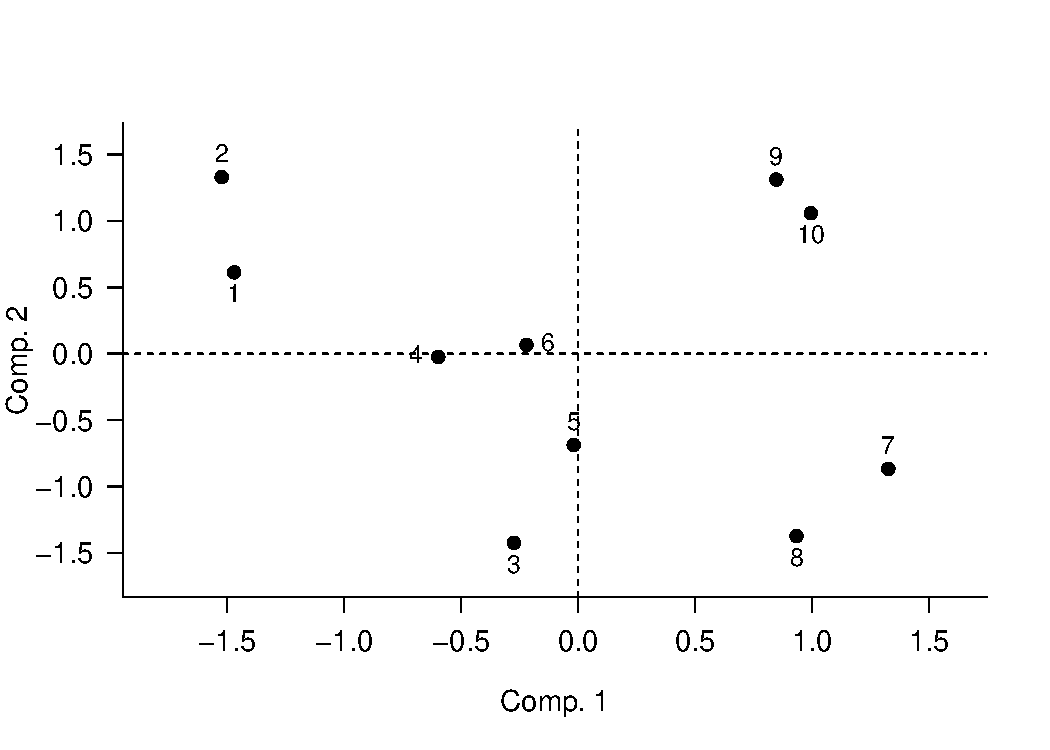
\includegraphics[width=0.65\linewidth]{figura07.pdf}
\caption{Score plot of the two first components in the \textbf{T} matrix}
\label{figura07}
\end{figure}

\begin{figure}[!ht]
\centering
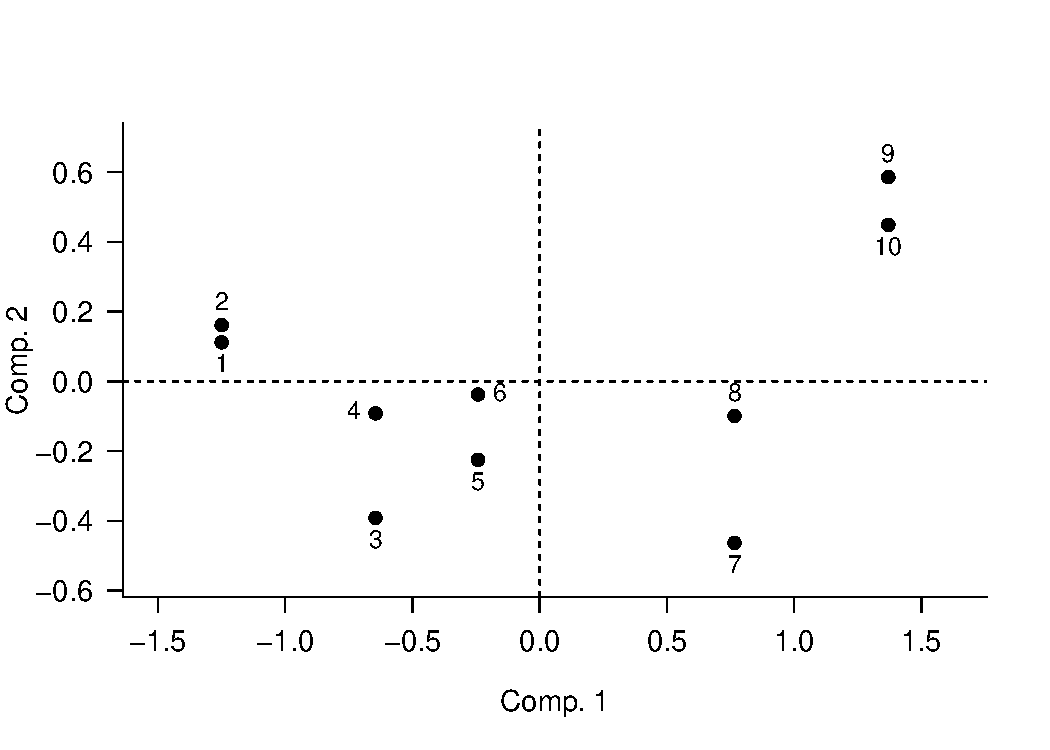
\includegraphics[width=0.65\linewidth]{figura08.pdf}
\caption{Score plot of the two first components in the \textbf{U} matrix}
\label{figura08}
\end{figure}

\autoref{figura07} shows how the 10 samples spread over the two first components. It can be seen how the samples evolve every two observations, from left to right, which seems reasonable attending to their different composition. \autoref{figura08} is similar, but related to the \textbf{y} scores. 

\vspace{15pt}
\begin{lstlisting}[basicstyle=\small, language=Python]
R> plot(fit, type="Wj", cex.axis=1.2, cex.lab=1.2, cex=1.2, 
+    las=1, bty="L")
R> plot(fit, type="Wk", cex.axis=1.2, cex.lab=1.2, cex=1.2, 
+    las=1, bty="L")
\end{lstlisting}

\begin{figure}[!ht]
\centering
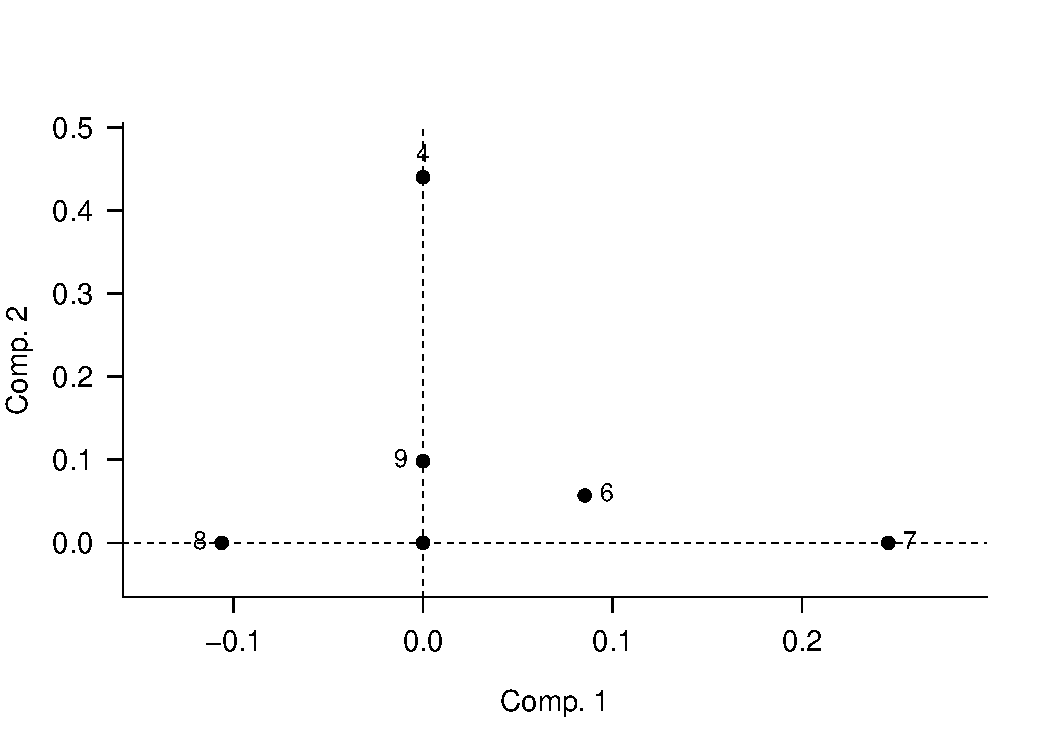
\includegraphics[width=0.65\linewidth]{figura09.pdf}
\caption{Weights Plot of the $\textbf{\text{W}}^{J}$ weights matrix}
\label{figura09}
\end{figure}

On the other hand, \autoref{figura09} presents the attributes and \autoref{figura10} the judges that help in predicting the \textbf{y} variable, for each of the two components. It can be seen that the first component of the attributes mode is related to attributes 7, 8 and 6 (in descending order in absolute values); whereas attributes 4, 9 and 6 are related to the second component. This can be also derived from \autoref{figura11}, which produces an equivalent graph. In this case, when trying to see what kind of relationship these attributes have with the judges’ mode, \autoref{figura12} provides easier-to-interpret results.

\begin{figure}[!ht]
\centering
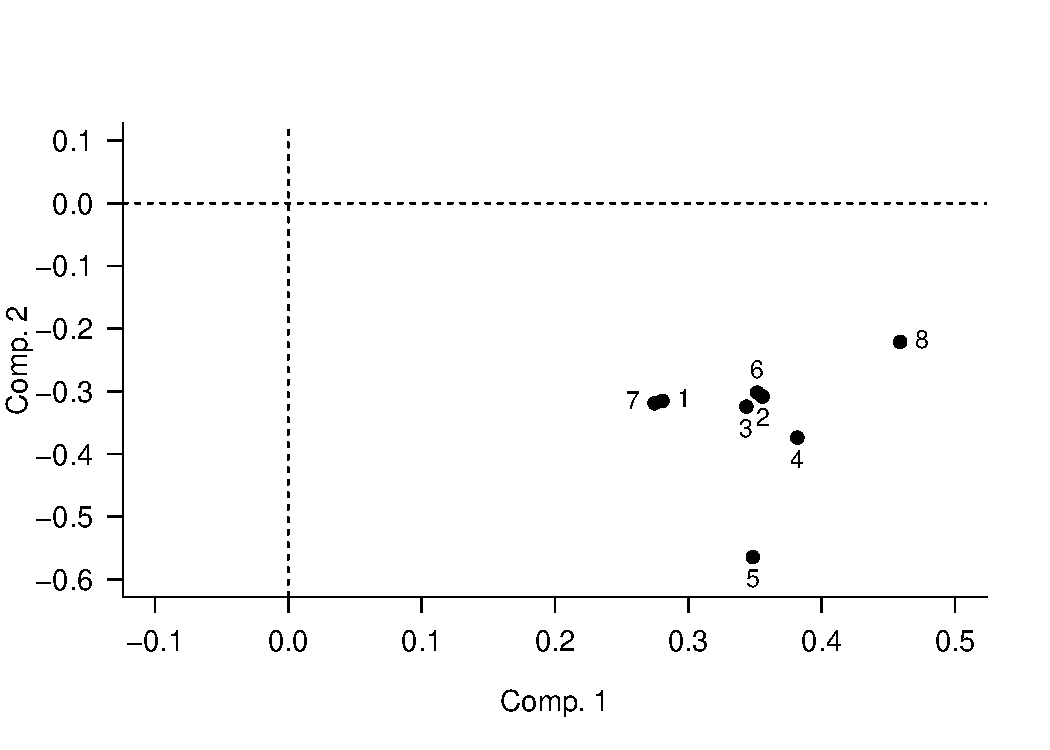
\includegraphics[width=0.65\linewidth]{figura10.pdf}
\caption{Weights Plot of the $\textbf{\text{W}}^{K}$ weights matrix}
\label{figura10}
\end{figure}

\vspace{15pt}
\begin{lstlisting}[basicstyle=\small, language=Python]
R> plot(fit, type="variables", cex.axis=1.2, cex.lab=1.2, 
+   cex=1.2, las=1, bty="L", lwd=2)
R> plot(fit, type="time", cex.axis=1.2, cex.lab=1.2, cex=1.2, 
+   las=1, bty="L", lwd=2, xlab="Judge")
\end{lstlisting}

\begin{figure}[!ht]
	\centering
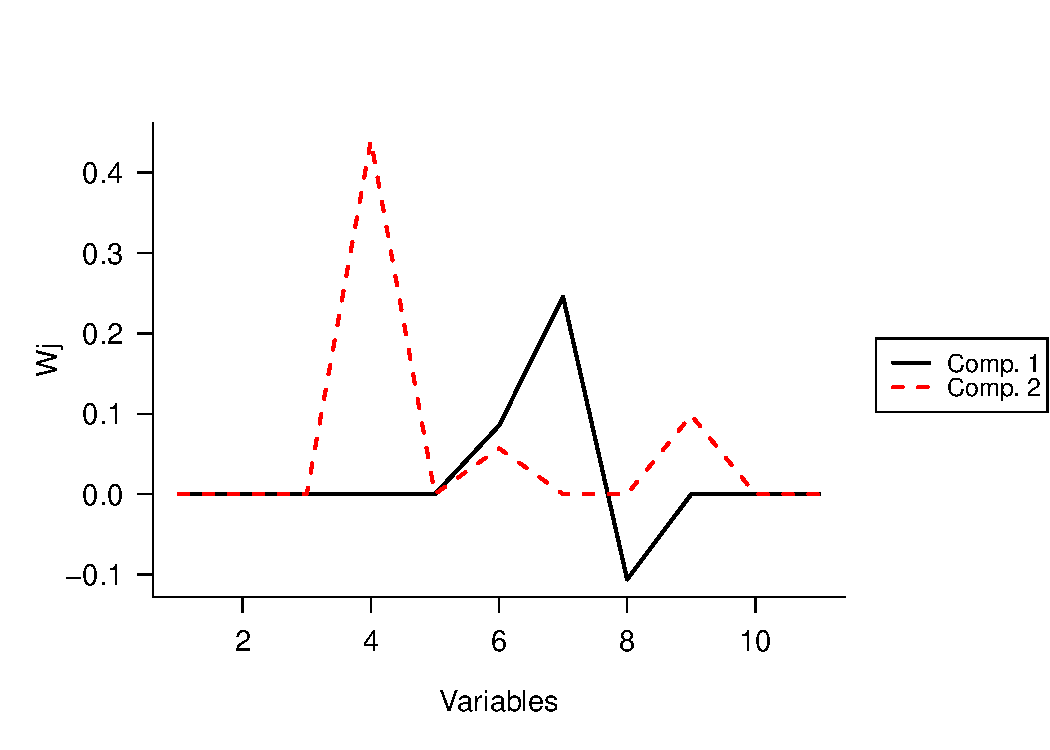
\includegraphics[width=0.65\textwidth]{figura11.pdf}
\caption{Plot of the second mode}
\label{figura11}
\end{figure}

It can be seen how, for the first component, there is approximately the same effect of all judges with respect variables 7, 8 and 6 (those related to the first component in the attributes mode) when trying to predict the salt content. In this case, since the judges’ weights show positive values, the higher the value of attributes 7 and 6, and the lower the value of attribute 8, the higher the salt content. For the second component, attributes 4, 9 and 6 are more influenced by judge 5, even though the rest of judges also have a similar effect on the salt content scoring (y variable). Since the weights of the judges’ mode are all negative for the second component, the higher the value of attributes 4, 9 and 6, the lower the salt content. In this case, \autoref{figura10} is less interpretable. However, depending on the case, one representation or another might provide easier-to-interpret results; so it is decided to keep both graphs in the package.

\begin{figure}[!ht]
	\centering
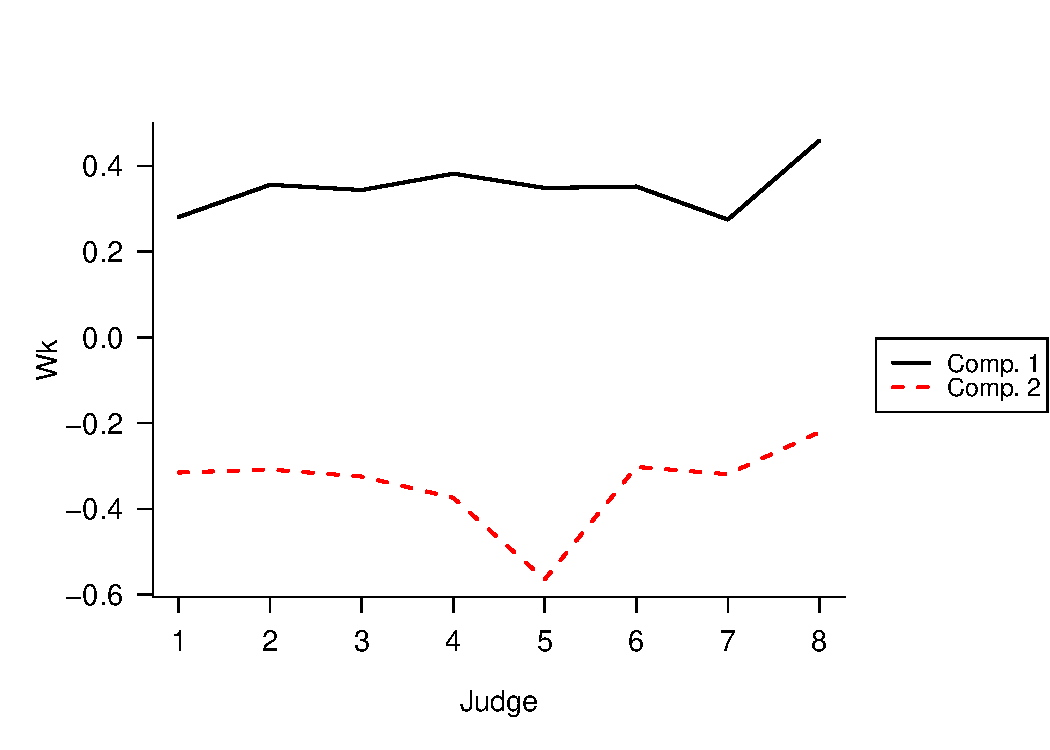
\includegraphics[width=0.7\textwidth]{figura12.pdf}
\caption{Plot of the third mode}
\label{figura12}
\end{figure}
\vspace{10pt}

As seen on these examples, all plots produced by the \texttt{plot.sNPLS} function are fully customizable, being able to change the titles, labels, orientation of labels, axis, size of the plot, etc., by using \textit{base} plot parameters such as \texttt{las}, \texttt{cex}, \texttt{bty}, etc. Since they are base \texttt{R} plots, they can be affected by all \texttt{par} options and also be combined in a single figure by using the \texttt{mfrow} and \texttt{mfcol} options or the \texttt{layout} function.

Finally, the \texttt{predict} function can be used to make predictions using new \textbf{\underline{X}} data. As explained before, it makes use of the coefficients matrix \textbf{B} computed by the \texttt{Rmatrix} function (\autoref{rmatrixf}). Here we use it to make a prediction from a new random \textbf{\underline{X}} array with 10 new observations (\autoref{output5}). This function also has an optional parameter, \texttt{scale}, which defaults to \texttt{TRUE} for controlling the final scale of the predictions (original scale vs. post-processing scale).

\vspace{15pt}
\begin{lstlisting}[basicstyle=\small, language=Python, morekeywords={array, sample, predict}]
newX <- array(sample(0:5, 10*11*8, replace = TRUE), 
+    dim = c(10, 11, 8))
predict(fit, newX)
\end{lstlisting}
\vspace{15pt}
\begin{lstlisting}[basicstyle=\small, backgroundcolor=\color{output}, numbers=none, label={output5}, language=Python, caption=Predictions of the model on new data \texttt{newX}.]
            Y.1
 [1,] 1.4196482
 [2,] 0.7819288
 [3,] 0.9619593
 [4,] 1.0523621
 [5,] 1.2585099
 [6,] 0.7243910
 [7,] 0.6458718
 [8,] 1.2693292
 [9,] 0.8194011
 [10,] 1.2753320
\end{lstlisting}

The output of the function is a \textbf{Y} matrix with the 10 predicted values.

\subsection{Performance}
The package offers a complete set of functions for tuning, fitting and interpreting $N$-PLS and sNPLS models. As tuning is a computationally intensive method, all cross-validation functions in the package allow the use of parallelization through the \textit{parallel} package and also use sparse matrices from the \textit{Matrix} package. This two optimizations allow for speedups of up to 20 times faster computation times compared to non-parallelized computations with dense matrices. The use of sparse matrices also alleviates the use of RAM memory which, in the case of large data sets, could be a limiting factor in some computers. \autoref{figura03} shows the improvements in computing times by using parallelization with different number of cores. As seen in the figure, the multicore scaling allows for tuning a model with a search grid length of 900 in an eight-core machine in less time than it takes to tune a model with a search grid of 90 in a single core running at the same speed.

\begin{figure}[hbtp]
	\centering
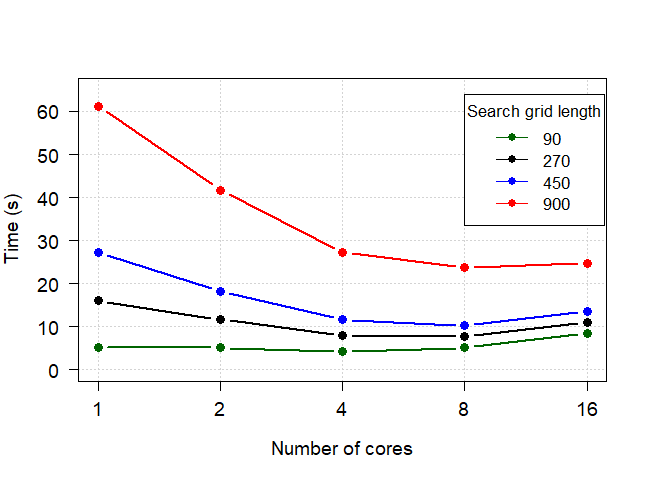
\includegraphics[width=0.65\textwidth]{figura03}
\caption[Computing times of \texttt{cv\_snpls} under different conditions of grid length and number of cores]{Computing times of \texttt{cv\_snpls} under different conditions of grid length and number of cores. The function scales efficiently up until 8 cores}
\label{figura03}
\end{figure}

The package also greatly benefits from the use of specialized Basic Linear Algebra Subprograms (BLAS) such as OpenBLAS, ATLAS or Intel\textsuperscript{\tiny\textregistered}  MKL, which can produce additional speedups of up to 10 times faster computation times \parencite{xianyi2014openblas, wang2014intel}. In this case, the potential benefit is left to the decision of the end user, that should install and link one of these BLAS libraries to \texttt{R}.

\section{Future work}
\label{packagedev}
The current version of the package is the 0.3.33, which is the 56th update of the initial package. At its current state, the package is fully functional, being able of fitting sparse and standard $N$-PLS models, efficiently performing cross-validation and repeated cross-validation and providing useful plots for the interpretation of results. The package recently incorporated generic base \texttt{R} functions for models such as \texttt{coef}, \texttt{summary} and \texttt{predict} and also has fixed all the detected bugs of the first versions of the software. According to the statistics given by \textit{CRAN}, the \texttt{sNPLS} package averages around 240 downloads per month and has accumulated more than 4500 downloads. These are similar statistics to the two other \texttt{R} packages for three-way analysis, so reception of our package seems to be great among the three-way community of \texttt{R} users.

For future versions of the package one of the priorities is including more options for the application of the penalization factor. Currently, the L1-penalty is determined by choosing the number of non-zero elements in $\textbf{\text{w}}^\text{J}$ and $\textbf{\text{w}}^\text{K}$, which can be determined by $K$-fold cross-validation or arbitrarily by the user. Ideally, the L1-penalty values should come from a continuous distribution, being able to take any value, not just discrete values as of now. Related to the application of penalty, we are also studying the possibility of adding an option for L0 penalty, This penalty can be applied using the hard-thresholding operator \parencite{zou2006adaptive}, so it should be straightforward to implement in future versions of the package.

Also the cross-validation procedure does not currently try all the possible combinations of the hyperparameter space, because when there is more than one component, all components are forced to have the same number of \texttt{keepJ} and \texttt{keepK} values. This constrain is only applied because of computational constrains, so different alternatives are being studied to be able to improve efficiency of the cross-validation procedure, thus removing the need for constraining the hyperparameter space. One of such alternatives, which will be implemented in future versions of the package will be the substitution of the grid search procedure for a random search procedure which has been demonstrated to be more efficient and also provide better estimates of uncertainty \parencite{bergstra2012random}.

Another addition regarding the tuning of the parameters and the cross-validation will be the possibility of personalizing the objective metric. Currently, the $RMSE$ is the only option for the optimization of the hyperparameter space. However, in the case of $N$-PLS-DA, other metrics related to classification methods such as missclassification rate or AUC \parencite{bradley1997use} would be more reasonable and should be implemented in future versions of the package.

Related to the optimization of the model by tuning of the hyperparameter space, alternative methods to cross-validation will be studied and implemented, such as information criteria based methods like Akaike information criterion (AIC) \parencite{akaike1974new} or Bayesian information criterion (BIC) \parencite{schwarz1978estimating}. These alternative methods should be much more efficient computationally, so they would be a great addition to the package.

We also have already experimented with the estimation of confidence intervals for the estimates based on resampling, so this will be another addition to the package in the upcoming versions. Related to this, the possibility of estimating the uncertainty in the variable selection procedure will be estudied and implemented if feasible.

Other planned addition is the modification of the plot function so that it creates objects with all the information about the plot instead of only producing them. This way, the user will be able to fully personalize their plots and also make their plots fully reproducible without the new of repeating a large analysis.

Finally, another objective is adding more useful functions to the package for providing a comprehensive framework for three-way analyses. Functions for performing Tucker and PARAFAC models like those already implemented in the \texttt{ThreeWay} and \texttt{PTAk} packages, more pre-processing functions and an extended documentation of all of them, including some vignettes, will be introduced in future versions of the package. Addition of other variable selection methods such as VIP scores and selectivity ratio for $N$-PLS is also planned. 
